\section{Z-ParaPack Design}\label{sec:design}
\subsection{PACKs and Lanes Organize Parallel File Updates}\label{sec:overview}
A PACK defines the contents that one synchronization must make durable; a lane manages the append permission needed to write those contents.
Z-ParaPack retains F2FS file mappings and block-validity semantics and gathers current writeback and pending mappings into each PACK.
The PACK appends current DATA and selected NODEs to its leased lane, with a terminal in the last selected NODE confirming completion.
Recovery validates and replays complete updates within the corresponding checkpoint generation.
Files have no permanent lane binding; subsequent updates can reuse lanes after lease release.

The system uses fifteen file-update lanes and one maintenance lane.
Ordinary non-inline DATA writeback uses file-update lanes by batch; \texttt{fsync}, \texttt{fdatasync}, and synchronous writes organize PACKs on these lanes.
A PACK's current DATA and related NODEs share its lane, although its closure can reference DATA from earlier writes on other lanes.
The maintenance lane handles NODEs outside commits, directories, quotas, and GC writes.

Figure~\ref{fig:architecture} traces parallel file updates through owners, lanes, and completion confirmation.
An owner coordinates synchronization; shared protection shards for the Segment Information Table (SIT) protect block validity.
Figure~\ref{fig:closure} expands closure selection and terminal confirmation for one PACK.
Figures~\ref{fig:lease} and~\ref{fig:recovery} explain append-permission reuse and commit recovery.

\begin{figure}[t]\centering
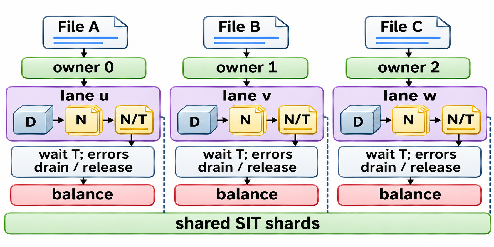
\includegraphics[width=.94\columnwidth]{./figures/redraw_architecture.pdf}
\caption{Independent files append DATA (D) and NODEs (N) through separate lanes, confirm the terminal (T) in the last NODE, drain, release leases, and run balance. Owners coordinate synchronization; dashed lines denote shared SIT protection. Files have no permanent lane binding.}\label{fig:architecture}
\end{figure}

\subsection{Mapping Closures Cover Updates Across Leases}\label{sec:closure}
Figure~\ref{fig:closure}(a) follows the $a'$, $b'$ example in Section~\ref{sec:joint}.
Earlier asynchronous writeback has written $a'$ and released its lease, but the mapping still awaits confirmation.
The current PACK includes this obligation together with the mapping obligation from writing $b'$.
It retains the NODE contents and marks that F2FS synchronization and roll-forward recovery require~\cite{r1}.

Mapping updates accumulate pending node identifiers (NIDs).
Synchronization first submits current DATA and records the corresponding NIDs (step~1), then captures the pending set and mapping-change sequence.
It adds the captured NIDs to the selection set (step~2).
The pending set can contain obligations from both earlier mappings and current writeback.
After waiting for the required DATA, the path deduplicates by NID and freezes the selection (step~3).
Per-inode pending and selection arrays grow as needed.
NIDs $a$, $b$ and their NODEs illustrate the process; updates can involve different numbers of nodes.

The path locks the entire selected NODE set and rechecks page identities, checkpoint generation, and mapping-change sequence (step~4).
Publishing a new mapping advances the sequence.
If this recheck detects a sequence change, the path abandons the PACK and falls back to a checkpoint as its dependencies require.
A stable selection enters the NODE append suffix in Figure~\ref{fig:closure}(b).
The DATA at $a'$ stays in place; current NODE writes confirm its mapping.
After a successful commit, the path clears pending entries only if the generation and sequence still match the snapshot, preserving obligations from later updates.

\begin{figure*}[t]\centering
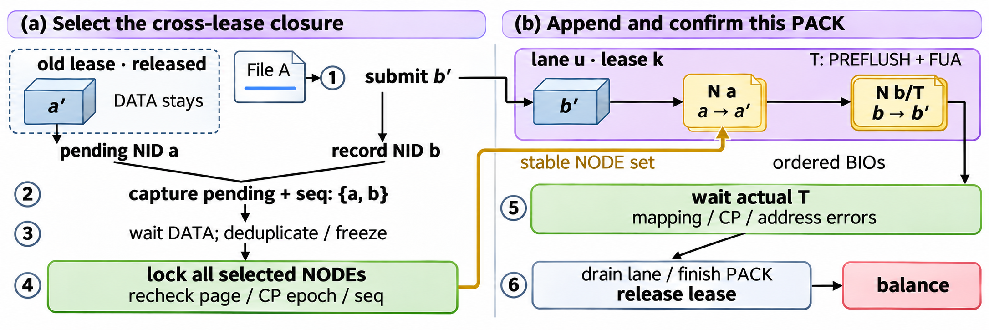
\includegraphics[width=.92\textwidth]{./figures/redraw_closure_terminal.pdf}
\caption{Cross-lease mapping closure and current commit. (a) Steps 1--4 submit current DATA, capture pending NIDs and sequence, wait and freeze a deduplicated selection, then recheck under locks. (b) Current $b'$ and selected NODEs share a lane; the last NODE carries T. Step~5 checks the actual T and errors; step~6 drains and releases the lease before balance. Earlier $a'$ stays in place; NIDs and node counts are illustrative.}\label{fig:closure}
\end{figure*}

\subsection{The Actual Terminal Defines Durable Completion}\label{sec:terminal}
Completion after distributing NODEs must refer to the current PACK.
The original fsync-node wait processes a list prefix by filesystem-wide node sequence number.
That prefix can include NODEs on other lanes, and the wait does not verify this PACK's terminal address.
Z-ParaPack tracks the page and block address of the last selected NODE and waits for that terminal.
This removes the wait point's dependency on NODEs from other lanes.
PACK NODEs retain node semantics; the block layer writes them to the lane through DATA-class block I/O units (BIOs).

In Figure~\ref{fig:closure}(b), current DATA $b'$ shares the lane with the selected NODEs.
N~a records the mapping for earlier DATA $a'$, while N~b/T records the mapping for $b'$ and carries the terminal.
On-disk next addresses connect the selected NODEs.
The last NODE uses that field for commit identity and a checksum.

The lane's ordered queue submits each BIO after its predecessor completes.
Current DATA and preceding NODEs use ordinary write requests.
The terminal requests a preflush (PREFLUSH) and force unit access (FUA).
When the device honors FLUSH/FUA semantics, terminal completion establishes durability for current DATA and selected NODEs.
It also confirms the closure's mappings for DATA from earlier asynchronous writeback.

Error handling follows the same completion boundary.
The queue records the first I/O error and completes subsequent requests with an error.
After the terminal page finishes writeback, synchronization also checks DATA/NODE mapping errors, checkpoint errors, and the terminal's submitted address.
Any failed check returns an error.
If an error follows submission of a NODE prefix, the path stops subsequent commits so that the prefix cannot connect to the next PACK's terminal.

After checking the terminal and errors (step~5), the path ends the PACK and waits for lane drainage.
Drain errors also affect the return status.
It then releases the lease (step~6), runs \texttt{balance}, and returns to the caller.
If the path cannot form a stable closure or acquire resources, it releases append protection and completes through a checkpoint as dependencies require.
The inode page and dentry recovery marks can cover inline DATA.
For eligible new small, empty, or inline files, the inode page can carry the terminal.
New files first exceeding inode coverage, and operations requiring global recovery metadata, use a checkpoint.



\subsection{Reusable Permissions Share a Physical Zone Ledger}\label{sec:lease}
Software lane reuse and physical zone release have different boundaries.
A lease identifies a lane and generation; allocation verifies permission before publishing an address.
After lease release, another update can use the lane.
Written zones can still occupy active or open resources, so foreground commits, asynchronous writeback, and maintenance share a physical ledger.
For each resource, the ledger maintains accounted occupancy plus reserved new occupancy within the device limit.

Physical operations reserve new occupancy before issuing device commands.
In Figure~\ref{fig:lease}, closing a partially written zone releases only open occupancy.
Successful finish or reset operations update the corresponding credits according to the resulting state.
GC relocation still coordinates with checkpoints, in-flight I/O, and read references; a failed operation cannot directly yield reusable credits.
Lease release returns software append permission without changing physical occupancy.

Commits and asynchronous batches release leases before entering maintenance that may depend on checkpoints or GC.
Subsequent file updates can therefore reuse their append state.
NODEs outside commits, directories, quotas, and GC writes use the reserved maintenance lane, leaving file-update append entry points available.
Both lane classes obey common physical limits; the maintenance lane adds no active or open capacity.

\begin{figure}[t]\centering
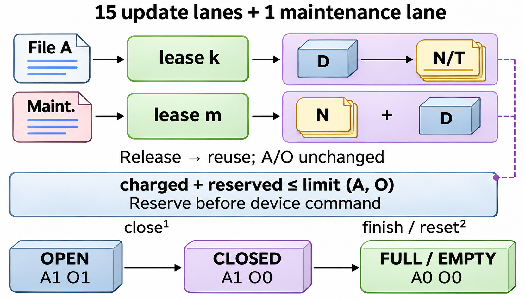
\includegraphics[width=\columnwidth]{./figures/redraw_lease_budget.pdf}
\caption{Lease release permits lane reuse; zone state determines physical occupancy. All lanes share active (A)/open (O) accounting and reserve new occupancy first. States follow successful operations: closing a partially written zone releases O; finish/reset updates A/O by resulting state. Dashed lines denote accounting. Lease and checkpoint generations remain separate.}\label{fig:lease}
\end{figure}

\subsection{Checkpoint Generations Scope Ordered Recovery}\label{sec:recovery}
Physical positions locate nodes after distributed appends; commit numbers determine replay order.
A checkpoint records the lane layout and on-disk recovery descriptors.
Within each generation, PACKs obtain globally ordered commit numbers from a shared sequence allocator.
Each inode acquires its synchronization mutex before reserving a commit number and holds it until the PACK ends.
PACKs for one file thus reserve numbers and complete in synchronization-critical-section order, while different files still append concurrently.

A commit number and checkpoint generation jointly identify an update.
Sequence allocation coordinates with checkpoints and resets after a successful checkpoint.
Before exhausting the sequence space, the system requests a checkpoint to establish the next generation.
Recovery checks both generation and commit identity so that reused numbers cannot identify the same set of commits.
Runtime request width leaves the recorded lane layout unchanged; remount scans the physical ranges in that layout.

Node chains define the contents that each terminal confirms.
Recovery collects candidate terminals and uses nonterminal NODE next addresses to build a successor-to-predecessor index that also records inode identity.
A terminal never supplies a predecessor entry for another chain.
For each candidate, recovery checks the recoverable generation, terminal format and checksum, and inode and lane identities.
It backtraces unique same-inode predecessors from the terminal to the chain head, then validates the chain forward to that terminal (Figure~\ref{fig:recovery}).
Ambiguous predecessors, self-loops, and out-of-range addresses invalidate the candidate.
A partial commit without a valid terminal also establishes no completion boundary.

In Figure~\ref{fig:recovery}, the physical scan encounters txn9 at B100, T200, and A300.
Index entries 100:300 and 200:100 let recovery backtrace from T200 to A300, then preflight A300$\rightarrow$B100$\rightarrow$T200 forward.
Recovery replays valid commits in commit-number order.
It finds the inode or reconstructs it from a valid inode image, validates the related NODE chain, and replays addresses and namespace state.
Multiple valid commits for one inode therefore retain commit order regardless of physical scan order across lanes.

\begin{figure}[t]\centering
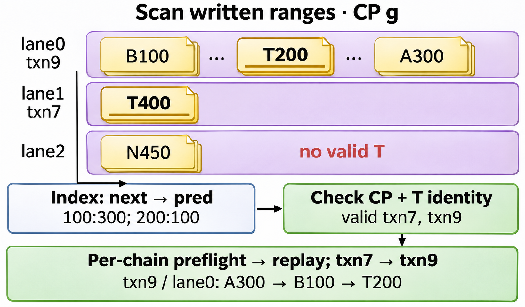
\includegraphics[width=\columnwidth]{./figures/redraw_recovery.pdf}
\caption{Physical scanning and ordered recovery. Only nonterminal NODE next addresses enter the predecessor index. After validating candidate terminals, recovery processes chains in commit-number order by backtracing, forward preflight, and replay. Partial commits without a valid T establish no completion boundary. Addresses and commit numbers are illustrative.}\label{fig:recovery}
\end{figure}

\subsection{Reusing Namespace Commits Completed by Checkpoints}\label{sec:namespace}
Namespace obligations, including parent-directory relationships, can still constrain file-content PACK commits.
Z-ParaPack associates these obligations with completed checkpoints so subsequent synchronization can reuse durable results without repeating a checkpoint for the same obligations.
New namespace changes invalidate the old proof.

A successful checkpoint publishes the proof.
With PACK replay and strict MAIN routing enabled, dirtying directory obligations advances a shared change generation.
A checkpoint snapshots that generation at its start and publishes the committed generation after success.
Synchronization uses the proof only when both generations match and are nonzero.
It also checks that generations have not exhausted their range, checkpointing has no error and remains enabled, and no forced checkpoint request awaits service.

Regular-file and directory synchronization check their respective commit conditions.
For a singly linked, unencrypted regular file, synchronization holds the inode synchronization guard and checks the checkpointed inode node, valid parent number, and shared generation under the inode metadata lock.
It then corrects the in-memory parent information.
Directory synchronization retains DATA writeback waits and checks for dirty state, in-flight writeback, and errors.
A clean directory with a valid proof reuses the completed checkpoint; other cases execute a checkpoint.
Both synchronization paths only read the proof.

\subsection{Implementation and Supported Paths}\label{sec:implementation}
Owners and SIT shards support parallel execution of the commit protocol.
Among owners that can request a file-update lane, synchronization favors the owner with the fewest unreleased application admission tokens.
The count includes queued and executing requests.
Ties favor the file's existing owner hint, while the lane lease still grants append permission.
Owner count, request-lane width, and SIT shard count have separate configurations.

We call the task initiating a DATA writeback batch its producer.
A producer with a valid batch lease can execute allocation callbacks directly, reducing cross-thread delegation.
Admission checks the task, file mapping, filesystem, lane, and generation, and excludes error, teardown, GC, and quota paths.
The callback disables task migration and retains curseg, SIT, and physical-zone locks.
Other cases use the existing local or owner-delegated path, and BIO submission follows existing owner rules.

On overwrite, SIT marks the new block valid and the old block invalid.
The system selects shared protection shards by section number modulo sixteen and acquires relevant shards in a fixed order.
Ordinary local updates take global read-side protection; segment allocation boundaries and global space-state transitions take exclusive protection.
The on-disk SIT layout remains unchanged.

The implementation uses a new format, log-structured (LFS) mode, and strict MAIN routing.
It integrates ordinary buffered writeback, file synchronization, and corresponding NODE, directory, quota, and GC writes.
Format or inode admission rejects unsupported combinations involving encryption, compression, verity, atomic/copy-on-write (COW), or pinned files.
Supported zoned direct-write paths can fall back to buffered writes; workload definitions follow the I/O paths that execute.
